%% EduGuard — IEEE Open Journal style manuscript (Overleaf-ready)
%% All numerical claims are locked to repository artifacts validated by
%% scripts/final_paper_experiments.py. Do not invent numbers when editing.
\documentclass[journal]{IEEEtran}
\usepackage{cite}
\usepackage{amsmath,amssymb,amsfonts}
\usepackage{algorithmic}
\usepackage{graphicx}
\usepackage{textcomp}
\usepackage{xcolor}
\usepackage{booktabs}
\usepackage{multirow}
\usepackage{url}
\usepackage{hyperref}

\graphicspath{{figures/}{../figures/}{../../artifacts/evaluation/paper/}}

\begin{document}

\title{A Lightweight Multi-Modal Tiny LLM Framework for Privacy-Preserving Academic Assistance in University Environments}

\author{
  \IEEEauthorblockN{Author Names}
  \IEEEauthorblockA{
    Affiliation \\
    Email
  }
}

\maketitle

\begin{abstract}
University teaching materials often mix public learning resources with protected examination content.
Centralizing raw exam questions for model training raises privacy and governance concerns, while cloud-hosted assistants may be unsuitable for offline or controlled campus deployments.
This paper presents \textbf{EduGuard}, an offline-oriented academic assistance framework that separates (i)~a lightweight Bloom's taxonomy sequence classifier based on Qwen2.5-0.5B with LoRA, (ii)~a Qwen2.5-1.5B multitask causal generator for target-level question rewriting, extractive-style question answering, and scientific summarization, and (iii)~role-aware retrieval with hybrid query/output screening over public and protected corpora.
The Bloom classifier is trained under simulated federated optimization (FedAvg and FedProx).
On the official Figshare Bloom held-out test set ($N{=}350$), the selected FedProx IID checkpoint (best validation round~20) achieves accuracy $0.8057$, macro-F1 $0.7982$, and quadratic weighted kappa $0.8493$, compared with $0.8314$ / $0.8252$ for a centralized 0.5B LoRA baseline evaluated in the same repository artifact.
The final multitask generator uses the locked \emph{v3} training formulation.
On a frozen multitask test split ($N{=}8321$), v3 reports Bloom target agreement $0.8880$ (macro-F1 $0.8768$) when scored by the merged 0.5B classifier, QA exact match $0.5784$ and token F1 $0.7854$ on SQuAD-derived items ($N{=}5285$), and ROUGE-1/2/L of $0.2491$ / $0.0573$ / $0.1496$ on PubMed-derived summarization ($N{=}1500$).
Rescoring the same generations with the selected federated classifier raises Bloom target agreement to $0.9518$ (macro-F1 $0.9443$); the repository explicitly records that the classifier is not human ground truth.
The 1.5B generator is deployed as a Q4\_K\_M GGUF artifact ($986{,}048{,}032$~bytes) with measured mean latency $0.6865$~s and $28.89$ tokens/s in the recorded micro-benchmark.
PrivacyGuard blocks $104/104$ synthetic student attack prompts in the current taxonomy evaluation, but also yields a benign allow rate of $0.0$ on $15$ benign prompts, indicating an unresolved utility--blocking trade-off.
We do not claim formal differential privacy for the deployed system.
\end{abstract}

\begin{IEEEkeywords}
Bloom's taxonomy, federated learning, LoRA, multitask language models, retrieval-augmented generation, educational NLP, local inference, privacy-aware systems
\end{IEEEkeywords}

\section{Introduction}
Bloom's taxonomy remains a standard vocabulary for describing cognitive demand in assessment design~\cite{bloom1956taxonomy,anderson2001revision}.
Automatically labelling exam questions and rewriting them toward a teacher-specified cognitive level can reduce authoring effort, but raising model capacity by shipping raw institutional question banks to a central server is often undesirable.
Federated optimization offers a training-time alternative in which clients exchange model updates rather than raw items~\cite{mcmahan2017fedavg,li2020fedprox,kairouz2021advances}.
Separately, campus assistants increasingly combine retrieval with local generation~\cite{lewis2020rag}, which requires clear role boundaries between public learning corpora and protected examination stores.

EduGuard is implemented as a multi-component system rather than a single end-to-end model.
A 0.5B sequence-classification head predicts Bloom levels and validates rewritten questions.
A distinct 1.5B causal model, trained under the repository's multitask \emph{v3} protocol, generates rewrites, answers, and summaries.
Retrieval uses local embeddings and FAISS indexes~\cite{johnson2019faiss}, and a hybrid PrivacyGuard screens student queries and outputs against protected content.
Formal differential privacy was explored in development artifacts but is \emph{not} part of the contribution claims of this manuscript, following failed utility outcomes under DP federated training and the absence of a production DP guarantee.

This paper answers a focused set of empirical questions that match available evidence:
\begin{itemize}
  \item \textbf{RQ1.} How accurate is the 0.5B Bloom sequence classifier under centralized evaluation?
  \item \textbf{RQ2.} How do FedAvg and FedProx compare under the tested IID and non-IID partitions, and which checkpoint does the selection rule designate?
  \item \textbf{RQ3--RQ4.} How does the locked 1.5B multitask \emph{v3} model perform on rewrite, QA, and summarization, including source$\rightarrow$target Bloom cells?
  \item \textbf{RQ5.} How do rewrite validation rates change when the selected federated classifier scores the same v3 generations?
  \item \textbf{RQ6--RQ8.} What local GGUF footprint is observed, and what empirical blocking behaviour does PrivacyGuard exhibit under the recorded suites?
\end{itemize}

\section{Related Work}

\subsection{Small and local language models for education}
Task-specific small language models can be competitive with larger cloud models on narrow educational tasks while keeping inference inside an institution~\cite{slm2026teammates,saur2026grading,tinyllm2024,localai2026}.
Reported advantages are typically in-domain: cross-domain transfer is weaker, and automatic LLM judges of question quality can disagree with expert ratings, which argues for human review rather than fully automatic educational claims~\cite{slm2026teammates,saur2026grading}.
Local hosting is an infrastructure and governance property~\cite{bogicevic2026rag,localai2026}.
It does not, by itself, constitute a privacy proof.
EduGuard follows this pattern with two local Qwen2.5 models~\cite{qwen2024technical}: a 0.5B sequence classifier and a 1.5B generator deployed as Q4\_K\_M GGUF.
Generalization beyond the training distribution is not separately tested here.

\subsection{Retrieval-augmented generation}
RAG grounds generation in retrieved passages~\cite{lewis2020rag}.
Educational uses include hardware-tiered campus RAG~\cite{bogicevic2026rag} and Bloom-structured assessment that conditions grading on retrieved course context~\cite{ragcognitive2025}.
Those studies do not show that retrieval itself prevents leakage of confidential exam text.
EduGuard uses a local FAISS index~\cite{johnson2019faiss} with BGE-family embeddings~\cite{xiao2024bge} and separate public and protected corpora.
A privacy-weighted re-ranking term exists in the retriever implementation; role gating of indexes is enforced independently of that score.
Retrieval quality (Recall@k, MRR) is not established by a complete benchmark in the current repository, so RAG is described as an implemented grounding path rather than as a measured retrieval result.
QA and summarization metrics in this paper use SQuAD-style exact match and token F1~\cite{rajpurkar2016squad} and ROUGE~\cite{lin2004rouge}.

\subsection{Automated Bloom classification}
Bloom labelling has been studied for learning objectives~\cite{li2022objectives}, exam questions with lexical and embedding features~\cite{mohammed2020tfidf,abduljabbar2015bloom}, transformers~\cite{waheed2021bloomnet}, and comparisons of classical models against prompted LLMs~\cite{bloomanalysis2025,crossbloom2026}.
A recurring limitation is weak transfer across datasets or phrasings~\cite{waheed2021bloomnet,crossbloom2026}.
Much of that literature uses the original six-category scheme (Knowledge through Evaluation).
EduGuard uses the revised labels Remember, Understand, Apply, Analyze, Evaluate, and Create~\cite{anderson2001revision,bloom1956taxonomy}.
The schemes are related; they are not treated as identical.
Ordinal agreement is reported with quadratic weighted kappa~\cite{cohen1968weighted}.

\subsection{Question generation versus question rewriting}
Bloom-conditioned generation can produce quizzes that teachers rate as usable~\cite{teachers2024quizzes}, and target-level adherence has been measured for prompted LLMs, often with weaker Apply or Create behaviour~\cite{bea2024questions,qgen2024strategies}.
Automatic quality metrics can diverge from expert judgement~\cite{qgen2024strategies,slm2026teammates}, and level-wise strengths of model-written answers are not fully consistent across studies~\cite{gpt4answers2024}.
Those papers mostly generate new items from a topic.
They do not evaluate the EduGuard teacher path: classify an existing question, rewrite it toward a specified target level, and re-score the rewrite with a separate classifier.
That re-score is an automatic check.
It is not a human rating.

\subsection{LoRA, federated optimization, and differential privacy}
EduGuard adapts both models with LoRA~\cite{hu2022lora}, not QLoRA~\cite{dettmers2023qlora}.
Quantization is applied after training, and only to the causal generator.
The classifier uses rank $32$ and $\alpha{=}64$; the v3 generator uses rank $16$ and $\alpha{=}32$.
These are different training configurations and should not be collapsed into one LoRA setting.
QLoRA results in adjacent teaching or classification tasks~\cite{teachinglora,spamqlora2026} and other PEFT methods~\cite{sktuning2024} are background, not a description of this pipeline.

FedAvg~\cite{mcmahan2017fedavg,konecny2016comm} and FedProx~\cite{li2020fedprox} are the aggregation methods actually implemented for the Bloom classifier.
Federated LoRA variants that vary rank per client or correct A/B aggregation bias~\cite{flexlora2024,lorafair2024} are not implemented.
In the locked 20-round IID comparison, FedProx test accuracy ($0.8057$) is close to FedAvg ($0.8000$).
Under the tested five-round Dirichlet $\alpha{=}0.5$ setting, FedProx ($0.4571$) does not exceed FedAvg ($0.5029$).
That observation is specific to statistical label skew and a fixed $\mu{=}0.01$.
It is not a claim about FedProx under systems heterogeneity, where the original FedProx study reports larger gains~\cite{li2020fedprox}.

Federated learning reduces the need to pool raw client text; it is not differential privacy~\cite{mcmahan2017fedavg,alrubaie2018privacy,kairouz2021advances}.
A DP-SGD FedProx run (Opacus, noise multiplier $1.0$, five IID rounds) reached test accuracy $0.1286$ and was not adopted.
DP-SGD is cited only as that negative experimental outcome~\cite{abadi2016dpsgd}.

\subsection{Research gap}
Prior work supports local SLMs, Bloom classification, Bloom-targeted generation, RAG, LoRA, and federated optimization as separate techniques.
The combination examined here is narrower: role-separated public and protected retrieval, a content-leakage screen that is not formal DP, a 0.5B revised-taxonomy classifier trained with simulated FedAvg/FedProx, and a distinct 1.5B multitask generator that rewrites an existing question to a teacher-chosen level and is checked by the classifier.
EduGuard is positioned as that integration, not as a new optimizer or a new privacy definition.

\section{System Architecture}
Figure~\ref{fig:arch} summarizes the verified components.
Teacher workflows may authorize protected exam indexes; student workflows are restricted to public retrieval scope in the role model.
For target-level rewriting, the teacher supplies a question and a \emph{target} Bloom level.
The 1.5B v3 generator produces a candidate rewrite.
The 0.5B classifier scores the cognitive level for validation and analysis.
Student assistance routes through authorization, PrivacyGuard screening, public-corpus retrieval, local generation, and output screening.
The classifier is not used as a generative rewrite model.

\begin{figure*}[!t]
\centering
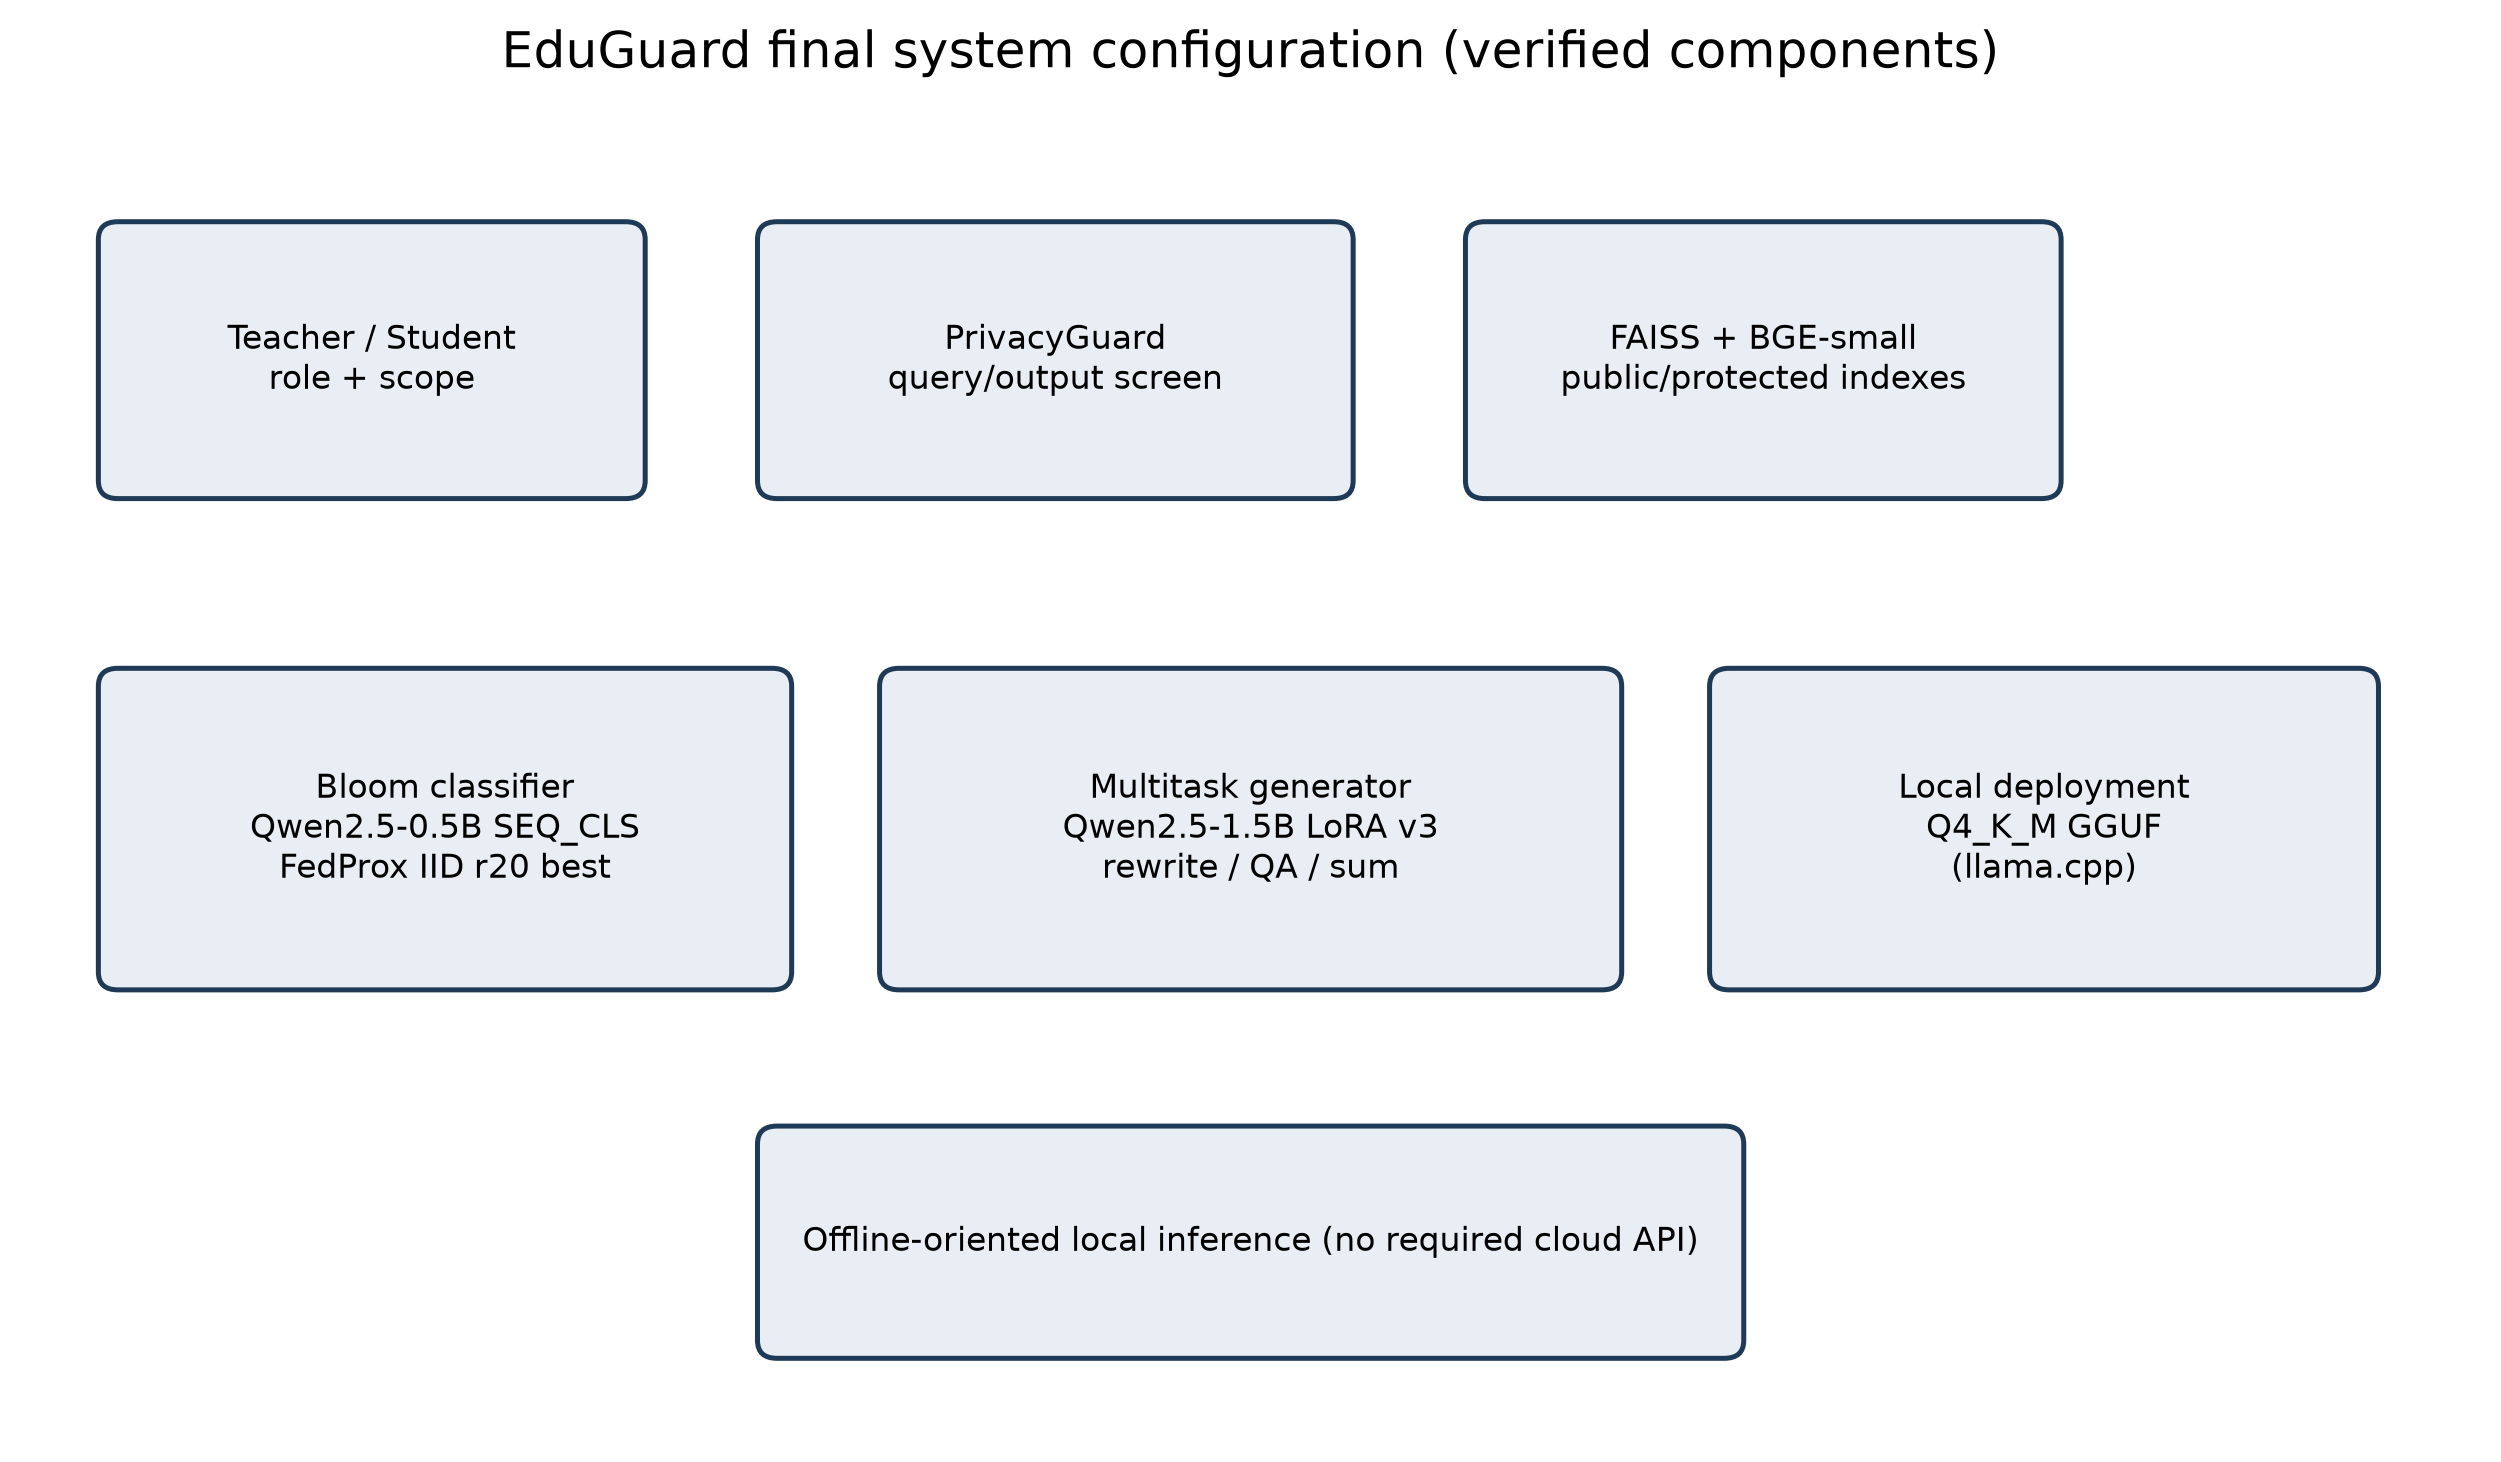
\includegraphics[width=0.95\textwidth]{fig01_system_architecture.png}
\caption{EduGuard final configuration: separate Bloom classifier, multitask generator, local retrieval, role separation, and PrivacyGuard. Schematic derived from the implemented modules.}
\label{fig:arch}
\end{figure*}

\section{Methodology}

\subsection{Bloom sequence classifier}
The classifier fine-tunes Qwen2.5-0.5B-Instruct as a six-way sequence-classification model with a score head and LoRA adapters (rank $32$, $\alpha{=}64$, dropout $0.1$).
The training split ($N{=}1631$) is imbalanced: Understand $640$, Remember $225$, Evaluate $199$, Apply $199$, Analyze $192$, Create $176$.
Class weights and label smoothing ($0.05$) are used in the federated training configuration.
Maximum sequence length for this classifier is $256$ tokens.
Classification is distinct from generation: the 0.5B model labels a question or a rewrite; it does not write the rewrite.

\subsection{Federated Bloom training}
We simulate eight teacher clients.
Algorithms: FedAvg and FedProx ($\mu{=}0.01$).
Partitions: IID and Dirichlet non-IID where executed.
Communication budgets include five-round diagnostics and twenty-round IID runs.
Checkpoint selection uses \emph{validation} accuracy (ties: macro-F1, then QWK).
Held-out Figshare test metrics are reported separately.
Federated learning here means federated optimization of LoRA/score parameters; it does not imply differential privacy, nor a mathematical impossibility of inference from updates~\cite{kairouz2021advances}.

\subsection{Multitask v3 generator}
The generator is Qwen2.5-1.5B-Instruct with multitask LoRA under the locked v3 dataset formulation.
Bloom rewrite supervision uses synthetic target-level transformations (policy v3); source Bloom labels are metadata for analysis and are \emph{not} supplied in the production-aligned generator prompt (question + target level only).
Training mixes Bloom rewrite, SQuAD-derived QA, and PubMed-derived summarization (Mix-A proportions in the v3 manifest).
Earlier multitask runs on synth\_v2 (`qwen05b_lora`, `qwen15b_lora`, `qwen15b_lora_sumfix`) are excluded from primary claims because of documented dataset/evaluation issues (format validity, answer-as-question leakage, weak Remember/Understand templates); see repository diagnosis reports.
The teacher path is classify, then rewrite to a chosen target level, then re-score the rewrite with the 0.5B classifier.
A trivial-transform rate is computed automatically.
No completed human ratings of Bloom alignment are available.
Context understanding and reasoning are prompt-conditioned behaviour inside the generator, not separate software modules.

\subsection{Protected corpus controls}
Student sessions are limited to the public index.
Teacher sessions may use an authorized protected scope.
PrivacyGuard screens queries and outputs with regex intent patterns, n-gram and longest-span overlap against protected text, and a semantic-concept check, with an auxiliary federated risk score.
This is a deterministic leakage screen.
It is not differential privacy and not a cryptographic proof.
The reported suite is the locked taxonomy evaluation ($104$ attacks, $15$ benign prompts), not an earlier $25$-case functional note that is not stored as a result artifact.

\subsection{Local quantized deployment}
Only the causal 1.5B generator is converted to Q4\_K\_M GGUF for llama.cpp inference.
The classifier remains a full-precision (FP16 export) sequence-classification model; dynamic INT8 was rejected because of accuracy collapse, and the classifier is not deployed as GGUF.
Offline-oriented configuration loads local model files and sets Hub offline flags.
Local execution removes a required cloud API for the intended path.
It is not itself a privacy guarantee; protection claims rest on role gating and PrivacyGuard.

\section{Experimental Setup}

\subsection{Datasets}
Figshare Bloom splits: train $1631$, validation $349$, test $350$.
Multitask v3 train total $6466$ (Bloom $2586$, QA $1940$, summarization $1940$); frozen test $8321$ with Bloom/QA/sum $1536$/$5285$/$1500$, byte-identical to the locked baseline test (SHA256 \texttt{1eb88cd5\ldots}).
Leakage checks in evaluation metrics report zero key/group overlaps between splits.
Bloom rewrite targets are synthetic; this is a central limitation.

\subsection{Metrics}
Classification: accuracy, macro-F1, QWK, within-one-level accuracy, severe-error rate, ECE.
Rewrite: classifier target agreement, fully-validated rate, semantic/cognitive rates, trivial-transform rate, $6{\times}6$ source$\rightarrow$target matrices.
QA: exact match and token F1.
Summarization: ROUGE-1/2/L.
Deployment: GGUF size, startup, latency, throughput, RSS/USS.
Privacy: attack block rate and benign allow rate.

\subsection{Environment}
Federated and multitask training/evaluation artifacts record GPU runs (including an RTX~4090 entry in v3 eval metadata).
GGUF micro-benchmarks record CPU-thread settings ($8$ threads, context $512$).

\section{Results}

\subsection{RQ1: Centralized Bloom classification}
On Figshare test ($N{=}350$), the centralized 0.5B LoRA evaluation artifact reports accuracy $0.8314$ and macro-F1 $0.8252$, versus TF-IDF+LinearSVC accuracy $0.7514$ and macro-F1 $0.7253$ in the same file.
A McNemar comparison against a 1.5B reference is recorded ($p{=}0.711071$, $n_{\mathrm{discordant}}{=}29$), but a complete 1.5B metric suite is not present on disk; we therefore do not claim a numerical 1.5B accuracy in the main table.
The 0.5B classifier is retained for footprint reasons consistent with the available evidence.

\subsection{RQ2: Federated comparison}
Table~\ref{tab:bloom} summarizes locked test metrics.
The selection procedure designates FedProx IID r20, best round $20$, with test accuracy $0.8057$ and macro-F1 $0.7982$.
FedAvg IID r20 selects best round $15$ (test accuracy $0.8000$).
Relative to centralized accuracy $0.8314$, FedProx trails by $2.57$ percentage points.
Non-IID five-round FedAvg at Dirichlet $\alpha{=}0.5$ drops to accuracy $0.5029$; FedProx non-IID $\alpha{=}0.5$ reaches $0.4571$.
Learning curves and best-versus-final comparisons are reused from the validated FL paper pack (Fig.~\ref{fig:curves}).
Live-evaluation ECE is $0.0537$; the training-run stored best-test ECE is $0.0565$ (disclosed disagreement).

\begin{table}[!t]
\centering
\caption{Bloom classifier test metrics on \texttt{figshare\_bloom\_v1\_test.csv} ($N{=}350$). FedProx ECE from live\_eval.}
\label{tab:bloom}
\begin{tabular}{lcccccc}
\toprule
Model & Acc & Macro-F1 & QWK & Within-1 & Severe & ECE \\
\midrule
TF-IDF + LinearSVC & 0.7514 & 0.7253 & 0.7471 & 0.8829 & 0.0657 & --- \\
Central LoRA 0.5B & 0.8314 & 0.8252 & 0.8794 & 0.9200 & 0.0371 & 0.0542 \\
FedAvg IID r20 (best r15) & 0.8000 & 0.7920 & 0.8412 & 0.8943 & 0.0486 & 0.0395 \\
FedProx IID r20 (best r20) & 0.8057 & 0.7982 & 0.8493 & 0.9086 & 0.0429 & 0.0537 \\
\bottomrule
\end{tabular}
\end{table}

\begin{figure}[!t]
\centering
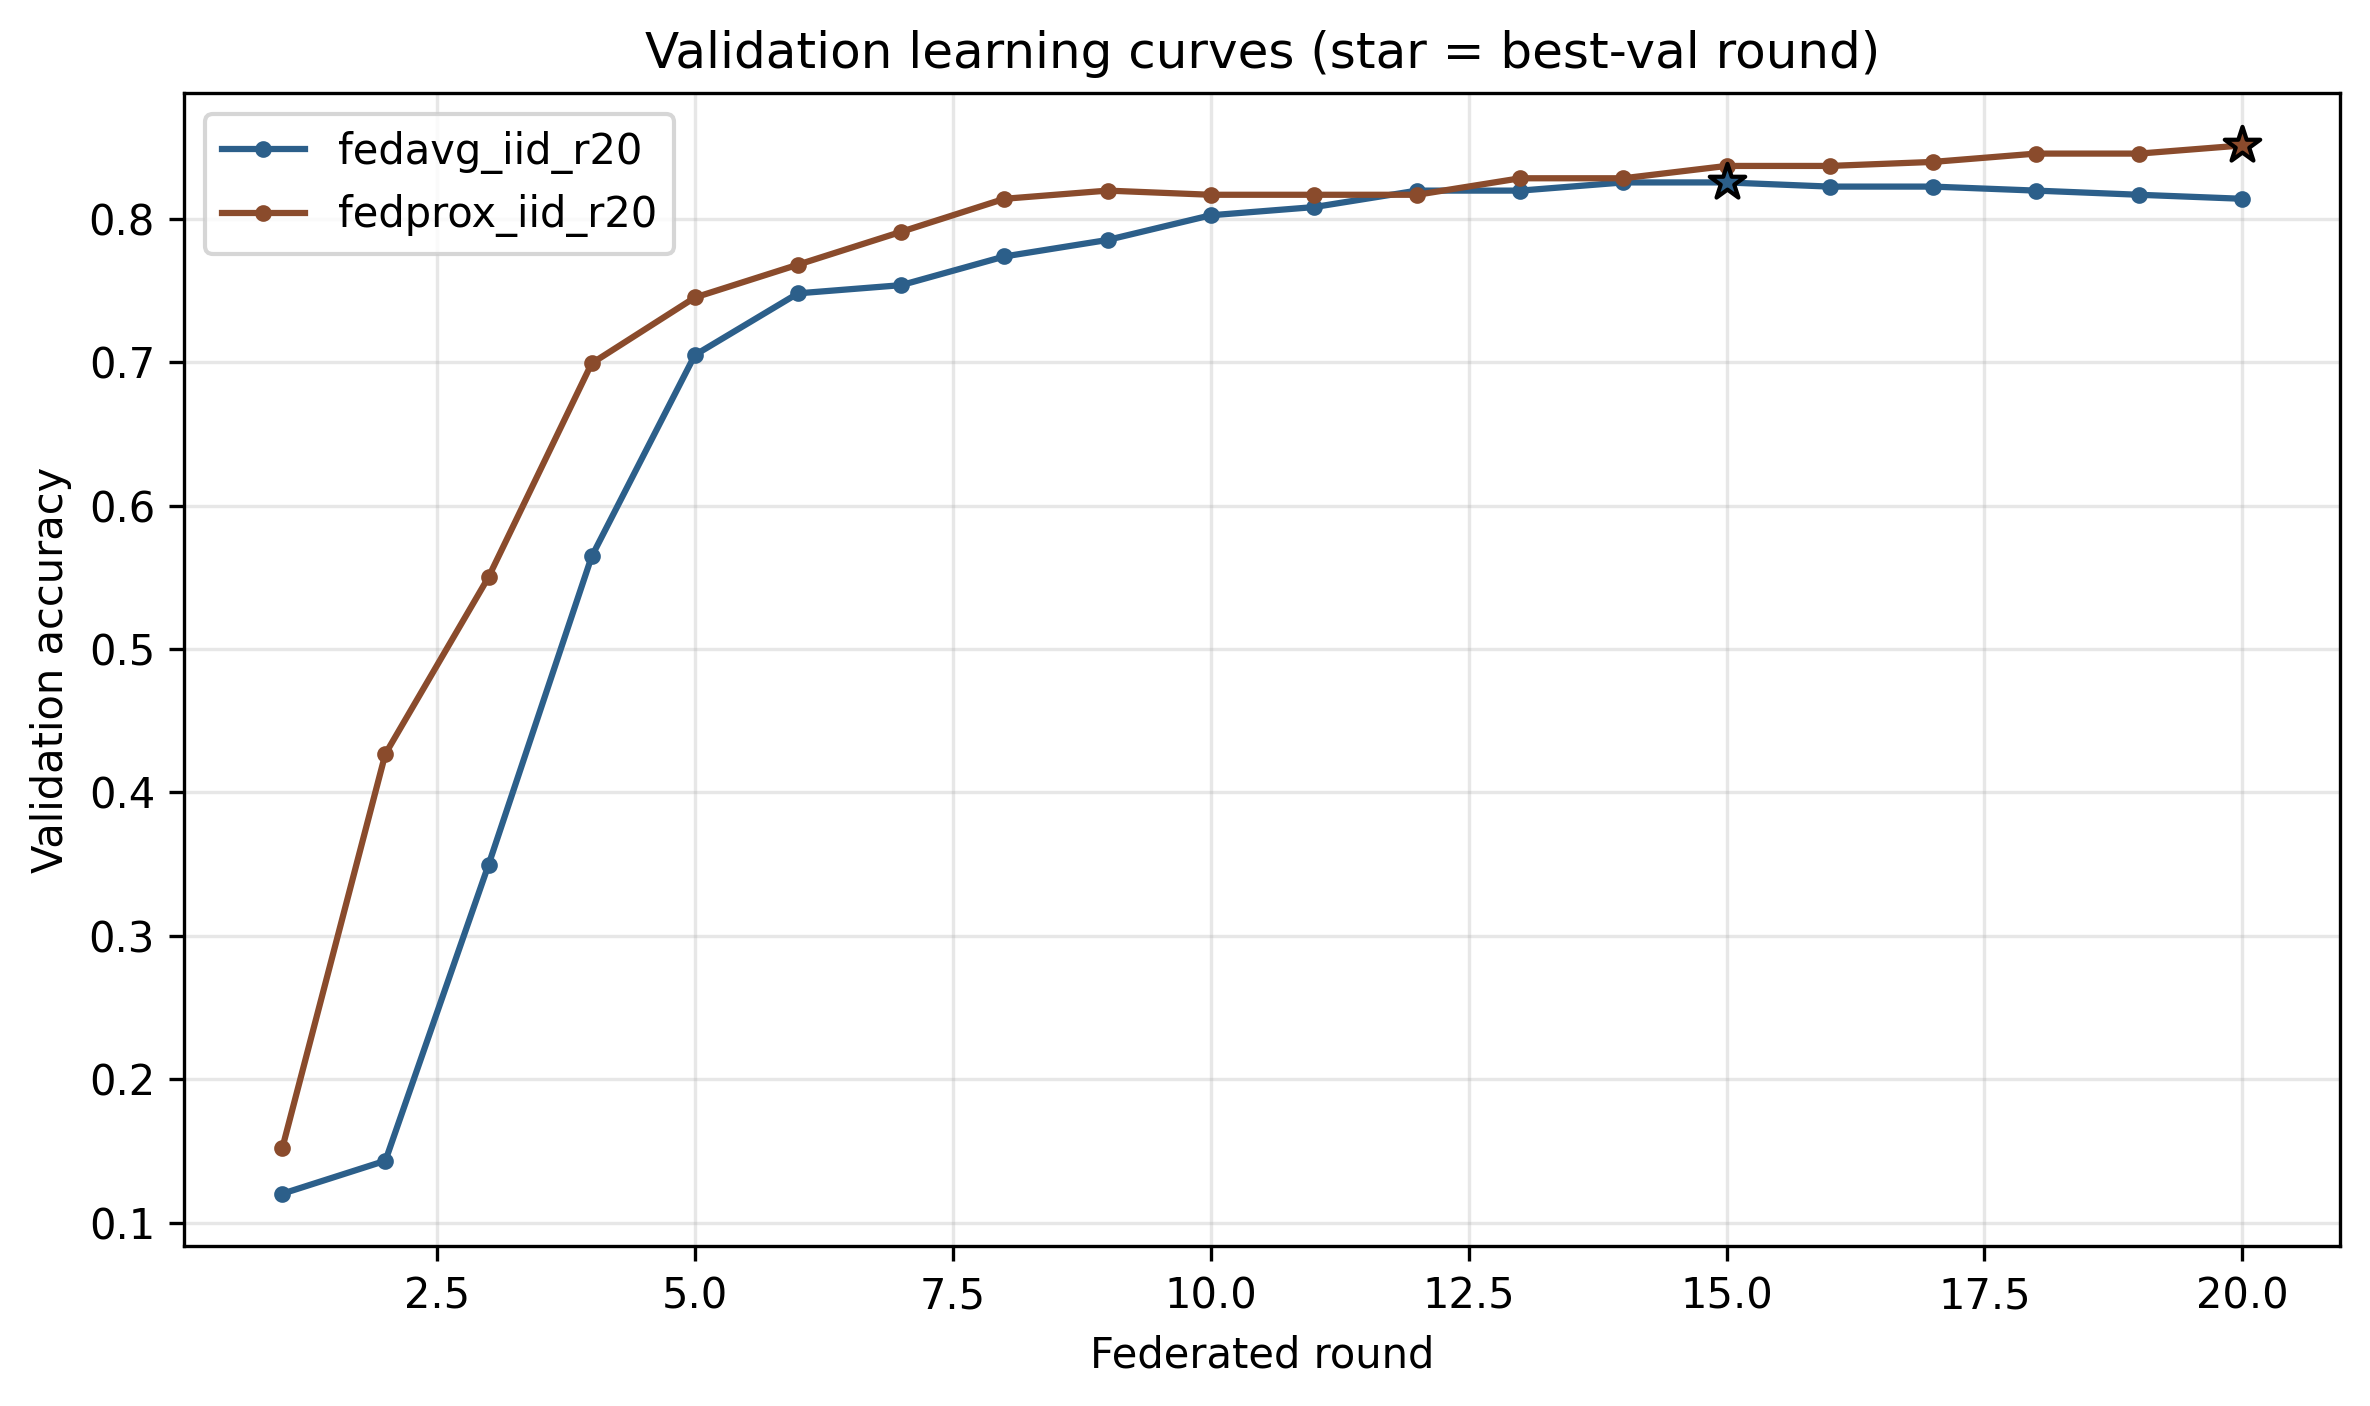
\includegraphics[width=\columnwidth]{fig03_fedavg_fedprox_learning_curves.png}
\caption{FedAvg vs FedProx validation learning curves (20-round IID runs; provenance: FL paper pack).}
\label{fig:curves}
\end{figure}

\begin{figure}[!t]
\centering
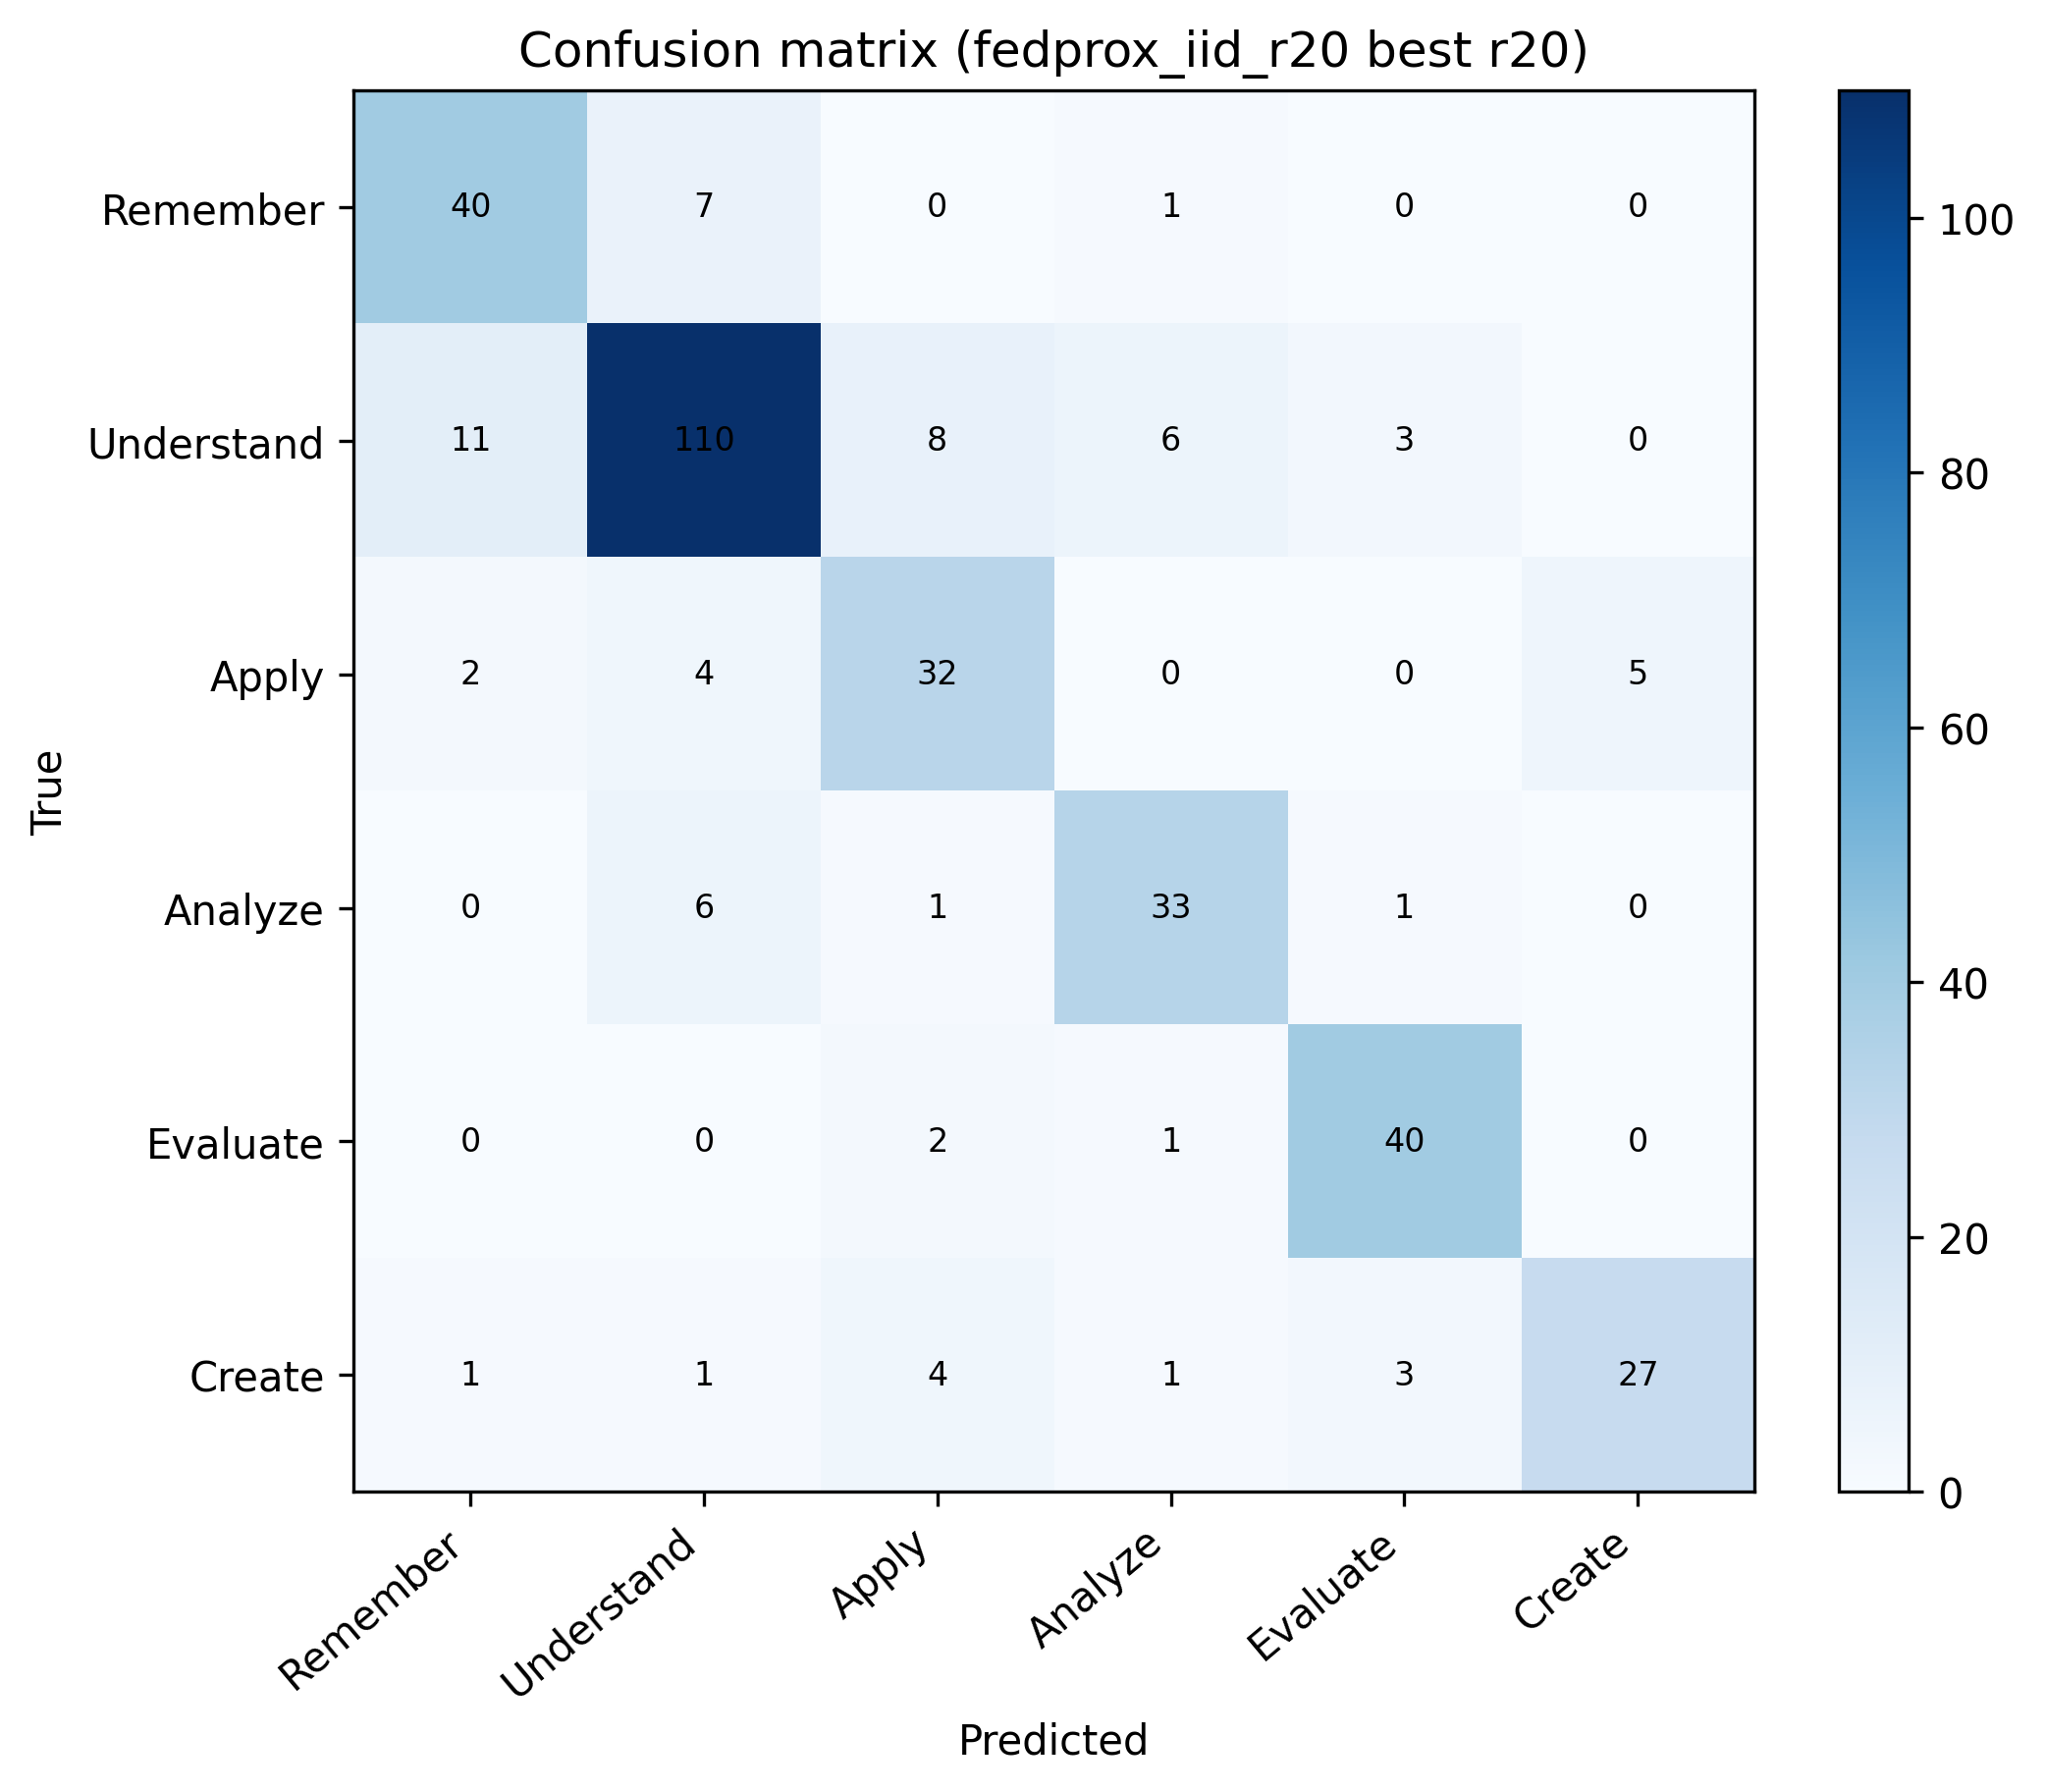
\includegraphics[width=\columnwidth]{fig02_bloom_confusion_matrix.png}
\caption{Confusion matrix for the selected FedProx IID r20 Bloom classifier on Figshare test ($N{=}350$).}
\label{fig:cm}
\end{figure}

\subsection{RQ3: Multitask v3 task performance}
Under the merged 0.5B classifier, Bloom rewrite target agreement is $0.8880$ (macro-F1 $0.8768$), fully-validated rate $0.7070$, semantic validity $0.8242$, cognitive validity $0.9954$, and trivial-transform rate $0.0013$ ($N{=}1536$).
QA yields EM $0.5784$ and F1 $0.7854$ ($N{=}5285$).
Summarization remains the weakest task: ROUGE-1/2/L $=0.2491/0.0573/0.1496$ ($N{=}1500$).
We do not claim uniform improvement across tasks.

A historical length ablation (\texttt{sumfix}; sequence length $1024$, new tokens $256$) increased summarization ROUGE and QA scores relative to primary v3 settings, but decreased fully-validated rewrite rate ($0.707\rightarrow0.557$) and cognitive validity ($0.995\rightarrow0.784$).
The primary v3 configuration ($512$/$128$) was retained to prioritize rewrite validation quality.
This is an observed configuration trade-off, not a causal claim beyond the tested settings.

\subsection{RQ4: Source$\rightarrow$target transformations}
Figures~\ref{fig:stacc}--\ref{fig:stfv} show $6{\times}6$ heatmaps for the integrated FedProx-scored matrix.
Performance is not uniform across cells.
Several upward transformations achieve high target agreement, while some downward transformations (for example, Understand$\rightarrow$Remember in the v3 matrix family) are comparatively weaker.
Aggregate scores alone would obscure these directional differences.

\begin{figure}[!t]
\centering
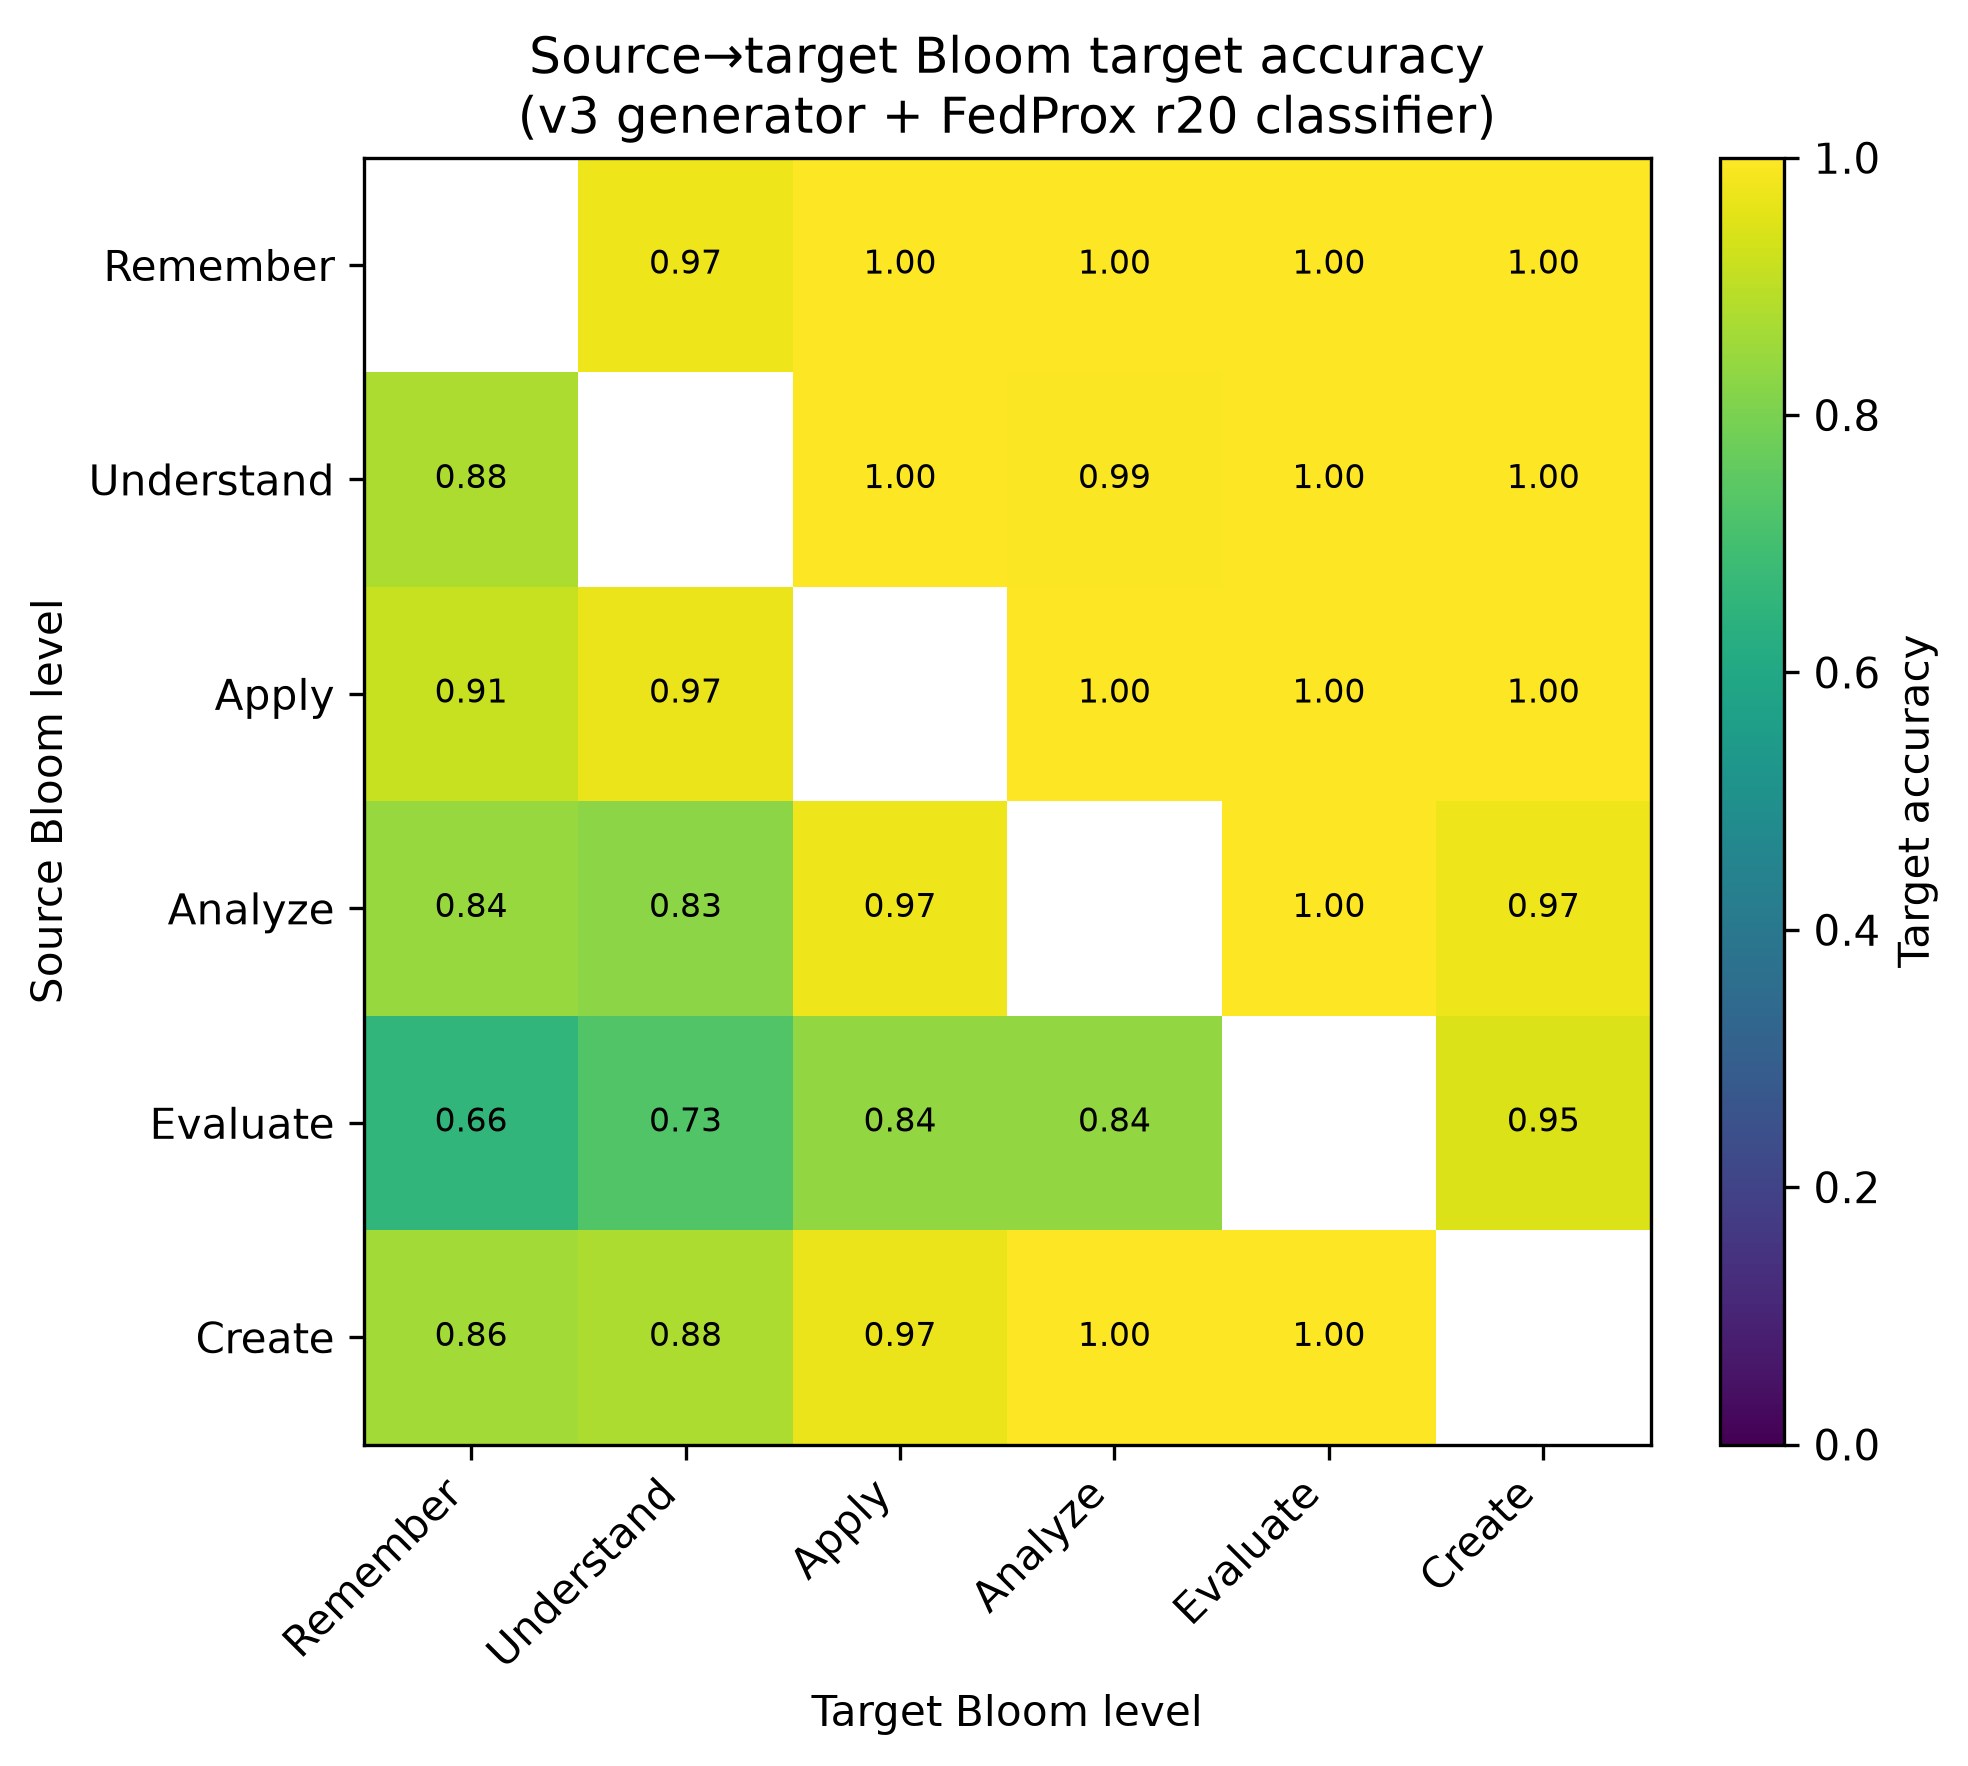
\includegraphics[width=\columnwidth]{fig04_source_target_accuracy.png}
\caption{Source$\rightarrow$target Bloom target accuracy (v3 generations scored by FedProx r20 classifier).}
\label{fig:stacc}
\end{figure}

\begin{figure}[!t]
\centering
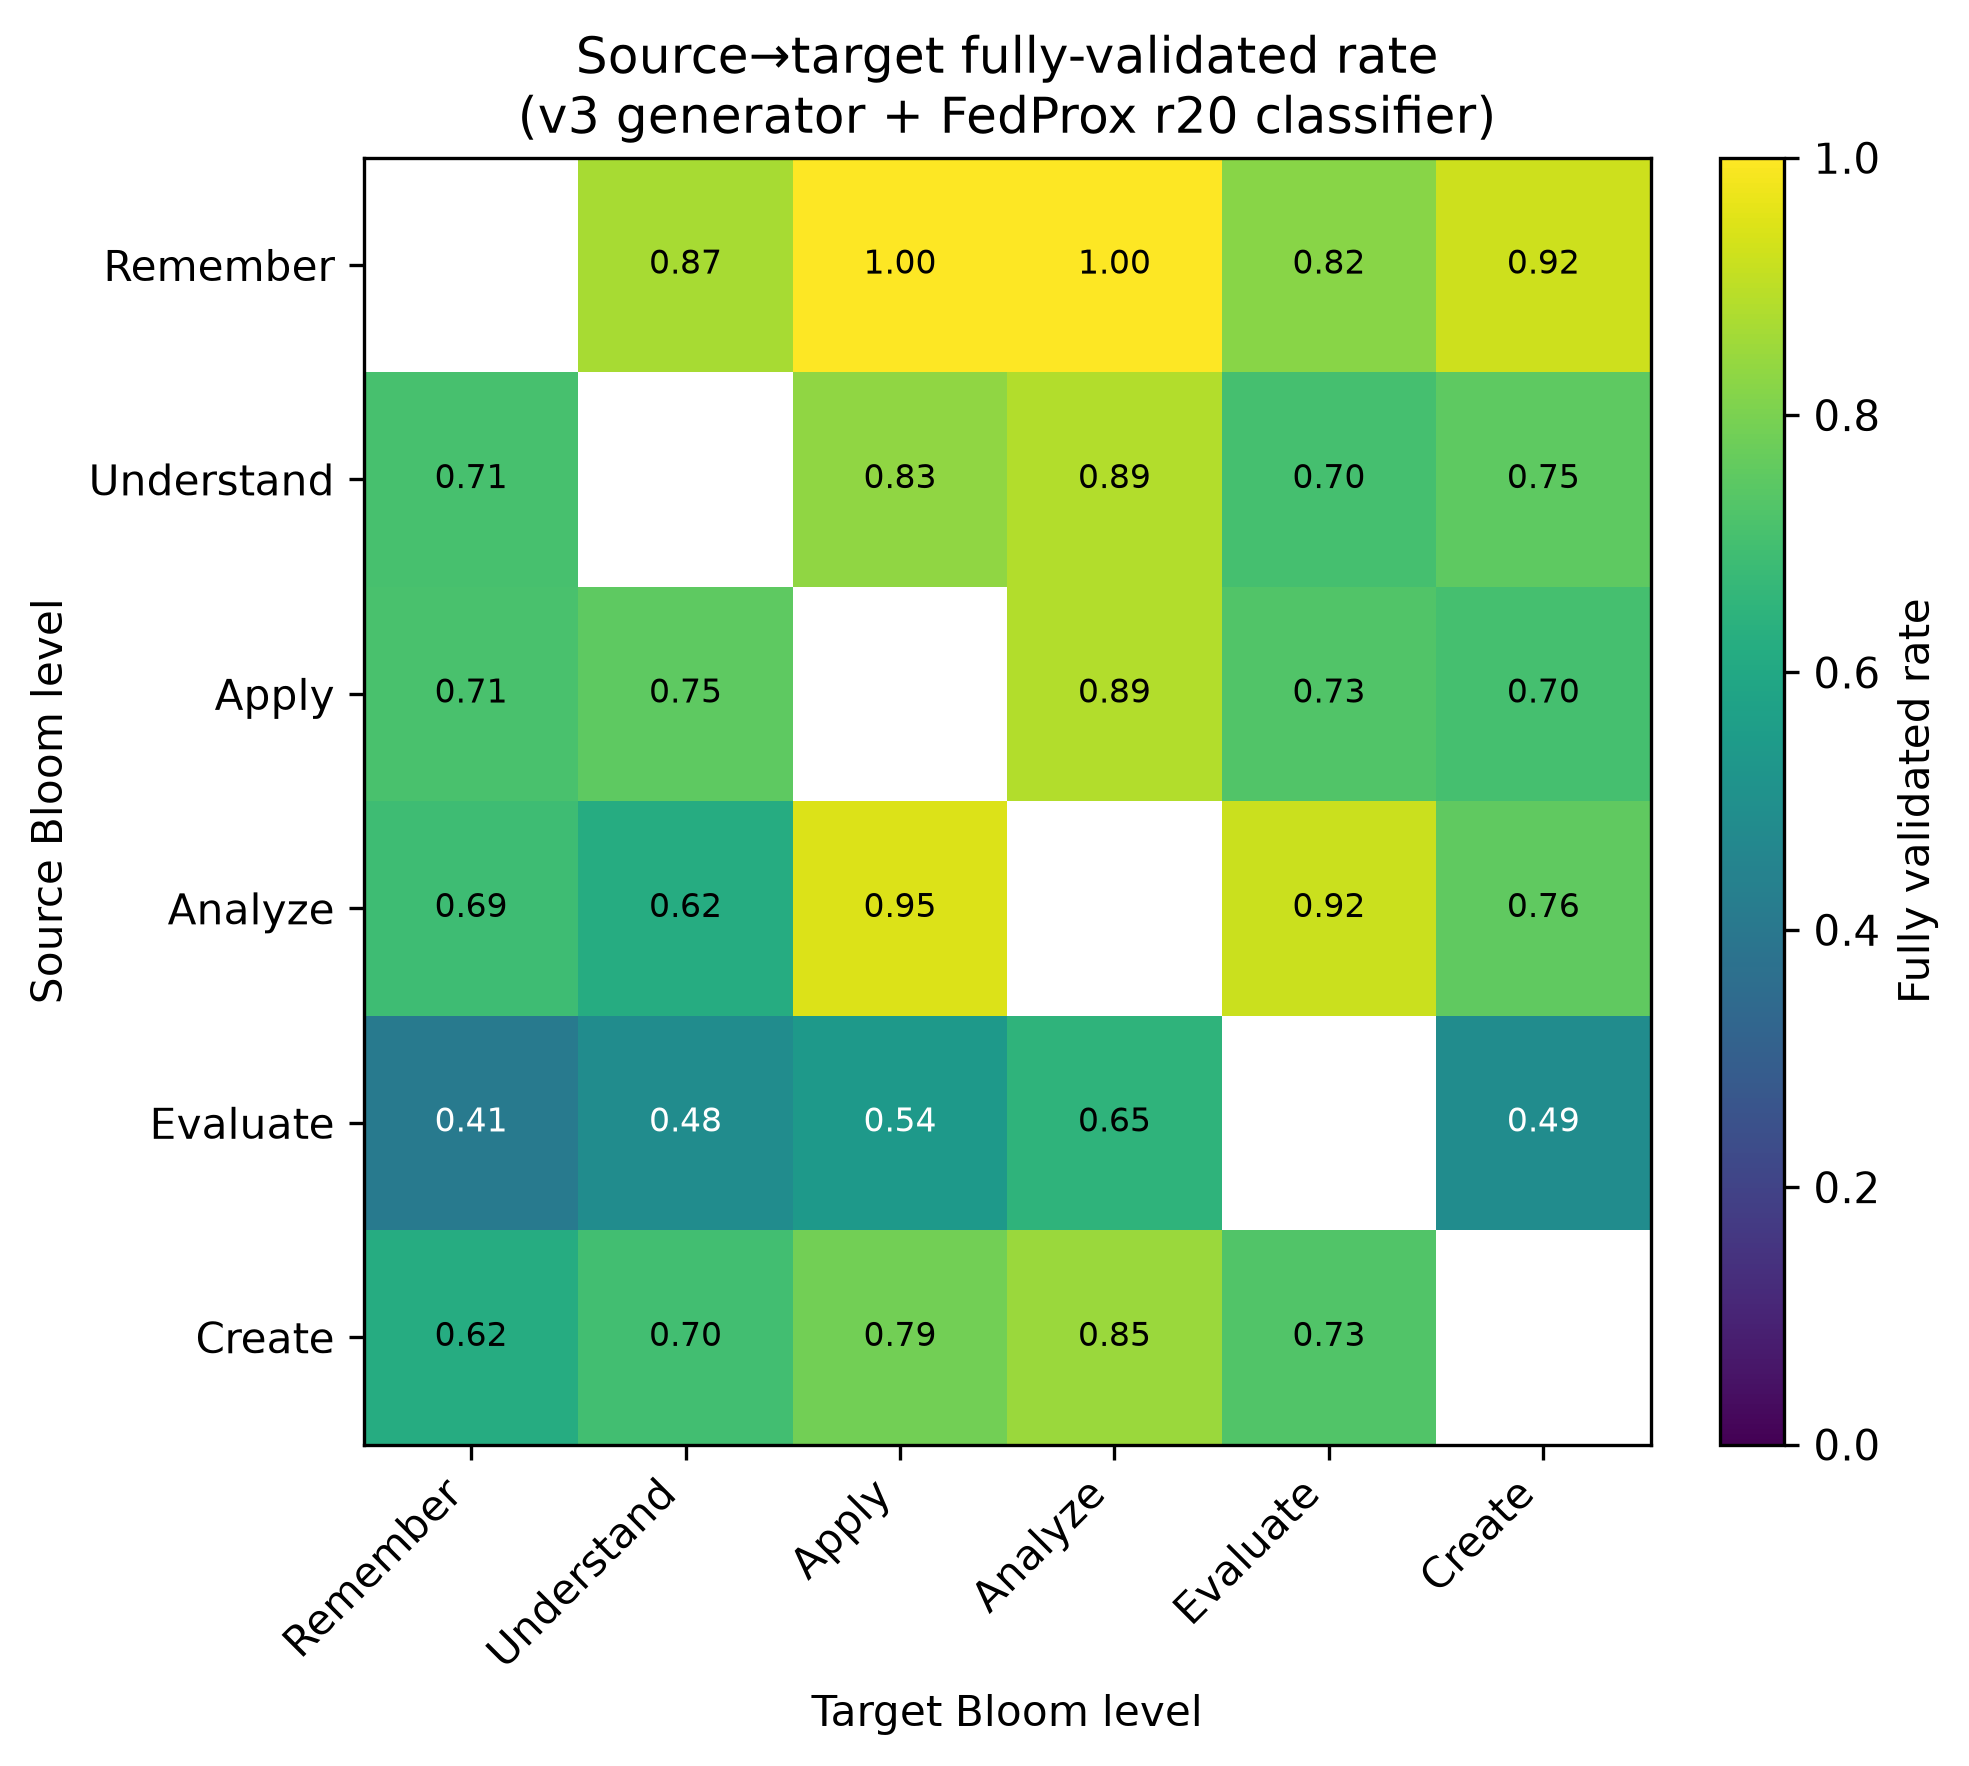
\includegraphics[width=\columnwidth]{fig05_source_target_fully_validated.png}
\caption{Source$\rightarrow$target fully-validated rates under the same integrated evaluation.}
\label{fig:stfv}
\end{figure}

\subsection{RQ5: Integrated federated classifier scoring}
Rescoring identical v3 generations with the FedProx classifier yields Bloom target agreement $0.9518$ (macro-F1 $0.9443$) and fully-validated rate $0.7624$.
QA and summarization metrics are unchanged because generations are unchanged.
The evaluation metadata sets \texttt{classifier\_is\_not\_ground\_truth=true}; automatic agreement is not a substitute for human educational judgement.
No completed human ratings exist in the repository rating files.

\subsection{RQ6--RQ8: Deployment, privacy, multimodal}
The Q4\_K\_M GGUF micro-benchmark reports size $986{,}048{,}032$~bytes, startup $0.687$~s, mean latency $0.6865$~s, P50 $0.6846$~s, P95 $0.7077$~s, mean throughput $28.8944$~tokens/s, peak RSS $1300.01$~MB, and USS $694.46$~MB.
PrivacyGuard taxonomy evaluation blocks $104/104$ student attacks (rate $1.0$) across reconstruction, leakage, jailbreak, paraphrase, partial-span, and semantic categories, while benign allow rate is $0.0$ on $15$ prompts---a severe utility cost under the current suite and thresholds.
Ablation over $1344$ attack cases shows regex-only blocking at approximately $0.524$, and full hybrid at $1.0$ with benign allow $0.0$.

\textbf{No complete quantitative EduGuard RAG benchmark was available in the current repository.}
A small academic QA smoke CSV ($n{=}10$) exists and must not be generalized.
OCR quantitative CER/WER benchmarks are likewise absent; multimodal support is an implementation capability with smoke-scale probes only.

\section{Discussion}
The strongest evidence-backed story is that a 0.5B Bloom classifier remains usable under FedProx IID training with a modest gap to centralized LoRA, while a separately trained 1.5B v3 multitask model provides rewrite-centred generation with secondary QA capability and weaker summarization.
Under the tested non-IID schedule, FedProx does not improve on FedAvg, which is consistent with using a single proximal coefficient on label skew rather than with the systems-heterogeneity setting in which FedProx was originally shown to help~\cite{li2020fedprox}.
Federated training is motivated by avoiding central pooling of raw teacher items in the experimental setup; it is not marketed as formal privacy.
The DP-SGD run is retained only as a negative utility result.
The PrivacyGuard results demonstrate aggressive attack blocking at the expense of benign availability---an honest systems finding rather than a success narrative.
Synthetic rewrite supervision and classifier-based validation limit educational conclusions.

\section{Limitations}
\begin{itemize}
  \item Synthetic Bloom transformation supervision; template memorization analysis in-repo covers synth\_v2, not a dedicated v3 report.
  \item Class imbalance and non-uniform source$\rightarrow$target difficulty.
  \item Weaker summarization ROUGE under the retained generation limits.
  \item Missing completed human evaluation ratings.
  \item Incomplete non-IID FedProx grid; five-round non-IID runs are not budget-matched to r20 IID.
  \item Formal DP validation history includes a failed gate and a later lock, but DP-FL test accuracy collapses to $0.1286$; no DP claim is made.
  \item No complete RAG/OCR quantitative benchmark.
  \item Some weight/GGUF binaries referenced under historical \texttt{D:\textbackslash Eduguard} paths may be absent in a given checkout.
\end{itemize}

\section{Conclusion}
EduGuard combines a federated 0.5B Bloom classifier (selected FedProx IID r20 checkpoint), a 1.5B multitask v3 generator, local retrieval controls, and Q4\_K\_M deployment for the generator only.
Reported metrics are taken from locked repository artifacts.
Future work includes human rating of rewrites, improved summarization without sacrificing rewrite validation, recalibrated PrivacyGuard thresholds for benign utility, and a proper retrieval benchmark.

\section*{Supplementary material}
The attachable bundle is \texttt{paper/attachment/}, rebuilt by
\texttt{scripts/build\_paper\_attachment.py}.
It contains the eight figures, the final tables, the experiment inventory,
the validation report, and the proof-status files for retrieval and PrivacyGuard.
Model weights are not included.

\section*{Data and Code}
Experiment inventory, validation report, and regeneration script:
\texttt{paper/final\_experiment\_inventory.md},
\texttt{paper/final\_validation\_report.md},
\texttt{scripts/final\_paper\_experiments.py}.

\bibliographystyle{IEEEtran}
\bibliography{references}

\end{document}
